\documentclass{article}
\usepackage{graphicx} % Required for inserting images
\usepackage[margin=1in]{geometry}
\usepackage{float}
\usepackage{url}
\title{Foundations of Data Science Final Project}
\author{Samira Rahman}
\date{October 2025}

\begin{document}

\maketitle

\section{Introduction}
This analysis explores RNA-seq gene expression data from The Cancer Genome Atlas (TCGA), focusing on understanding expression variability across different sample types, including metastatic, primary tumor, and solid tissue normal samples. The dataset contains normalized count data for hundreds of genes across multiple patient samples.

For this project, two genes were selected for deeper analysis:
\begin{itemize}
    \item \textbf{\textit{ENSG00000000419.13} (Gene1)}: a gene associated with cellular metabolic and structural functions.
    \item \textbf{\textit{ENSG00000000460.17} (Gene2)}: another gene showing moderate to high expression variability across tumor samples.
\end{itemize}
\noindent
Studying these genes helps illustrate how expression differs across cancer sample types, providing biological insights into transcriptional changes associated with tumor progression and metastasis.


\section{Methods}
All analyses were performed using \textbf{R version 4.5.1}. The following R packages were used:
\begin{itemize}
    \item \textbf{ggplot2 (v4.0.0)}: for generating histograms, scatter plots, violin plots, and bar charts.
    \item \textbf{ComplexHeatmap (v2.24.1)}: to create annotated heatmaps for multi-gene visualization.
    \item \textbf{circlize (v0.4.16)}: as a dependency for ComplexHeatmap color mapping.
    \item \textbf{xtable (v1.8.4)}: LaTeX compatible output formatting.
\end{itemize}
\noindent
The RNA-seq \textbf{count matrix} and associated \textbf{metadata file} were read into R. Counts were extracted for two specific genes, converted to numeric vectors, and combined with the metadata covariate \textit{sample\_type}. Visualizations were saved as PNG files. Summary statistics (mean, median, standard deviation, minimum, and maximum) were calculated for both selected genes and formatted as a LaTeX table for this document.


\section{Results}
A series of plots were generated to explore and visualize expression trends:

\subsection{Histogram}
This histogram shows the \textbf{distribution of expression counts} for the gene \textit{ENSG0000000419.13} across all samples. Most samples have low to moderate expression levels, with a sharp peak around lower count values and a long right tail. This right-skewed distribution indicates that while most samples express this gene at low levels, a few exhibit very high expression, suggesting potential overexpression in certain tumor samples.

\begin{figure}[h]
    \centering
    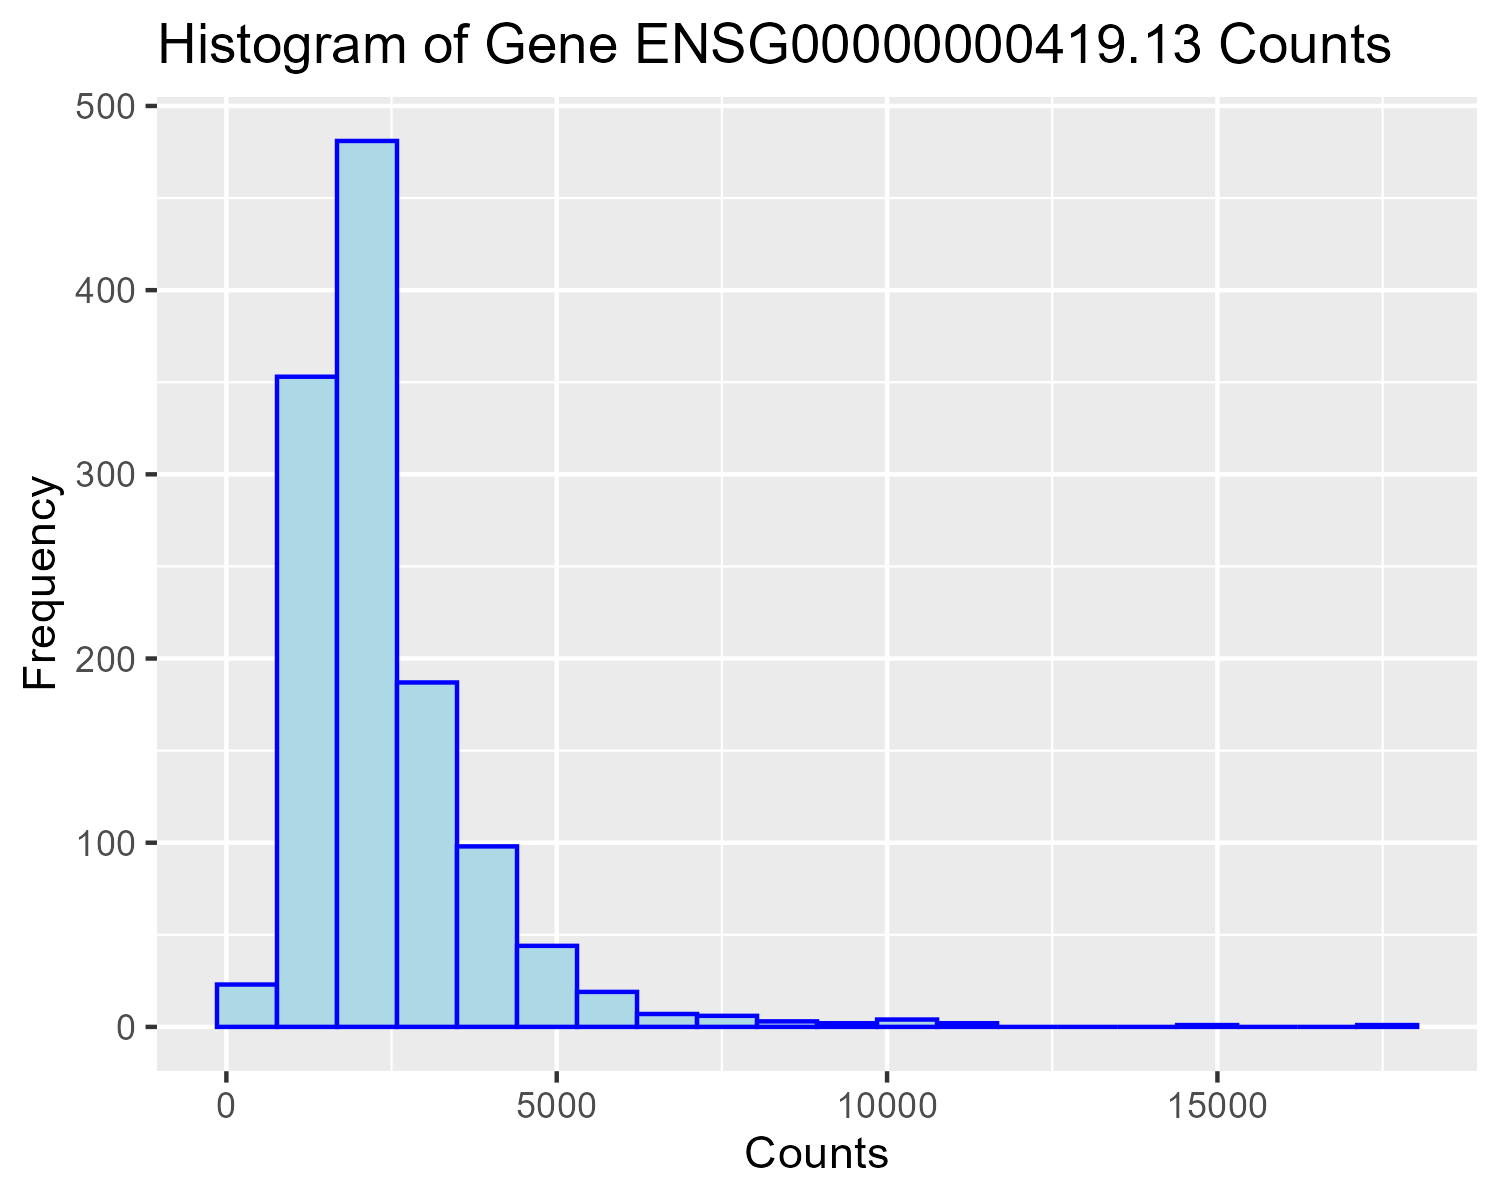
\includegraphics[width=0.6\textwidth]{final_project_histogram.png}
    \caption{Histogram of Gene ENSG00000000419.13 Counts.}
    \label{fig:histogram}
\end{figure}

\subsection{Scatter Plot}
The scatter plot comparing \textit{ENSG00000000419.13} and \textit{ENSG00000000460.17} showed a positive correlation between their expression levels across samples, suggesting potential co-regulation or shared biological pathways. The regression line with confidence interval (gray shading) supports this trend.

\begin{figure}[H]
    \centering
    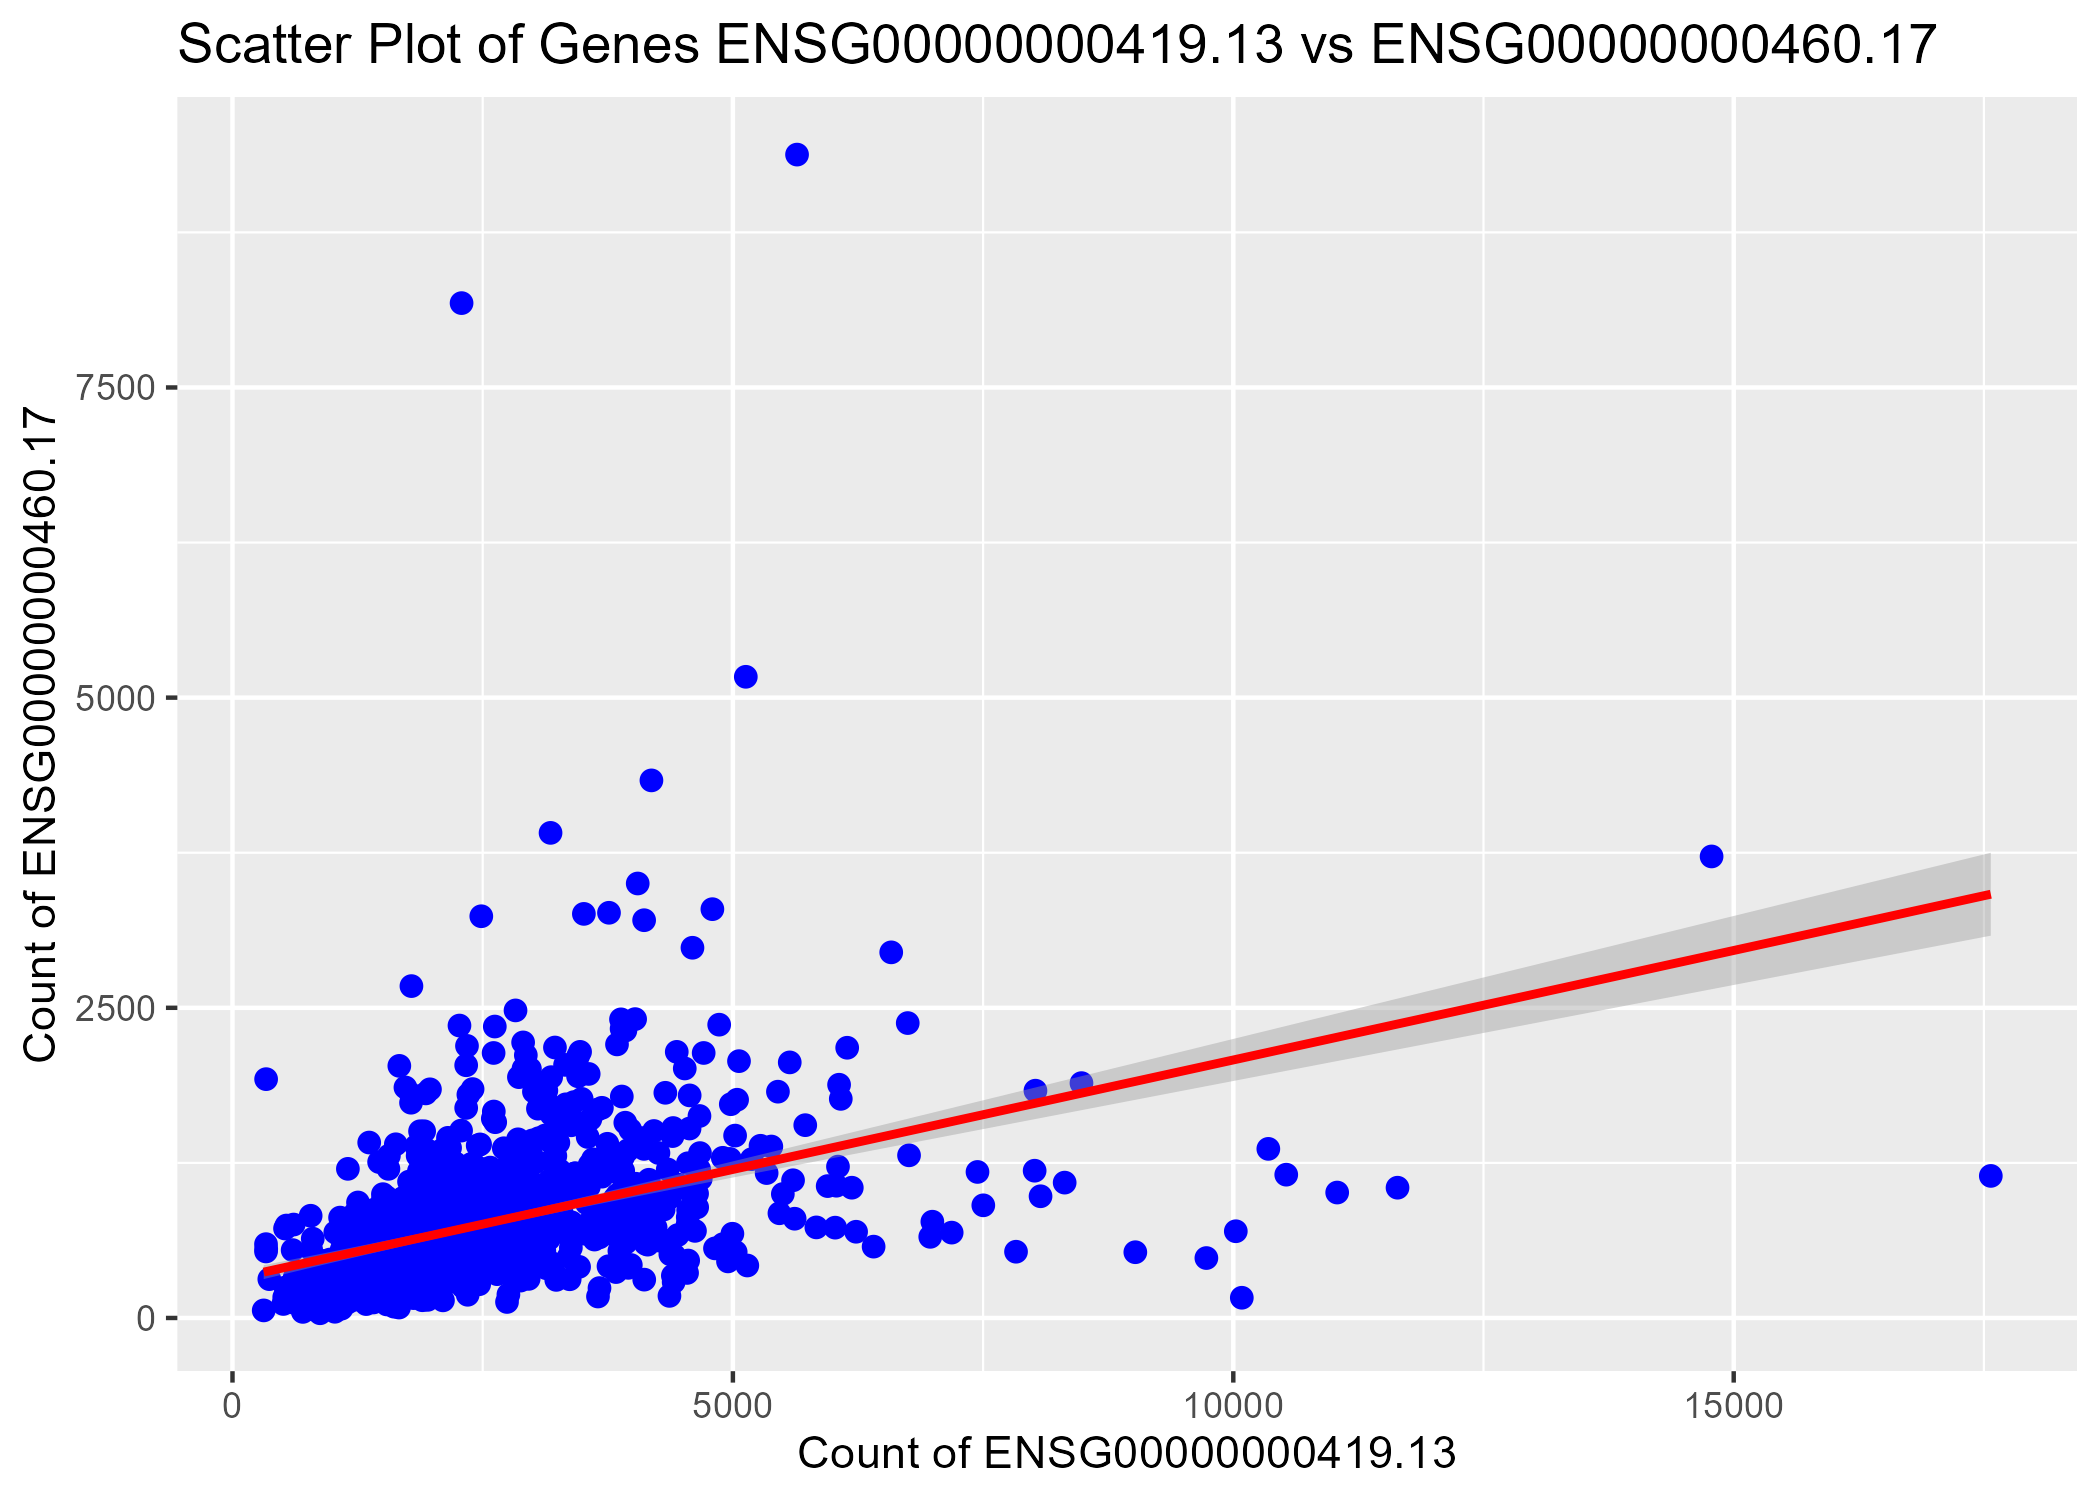
\includegraphics[width=0.7\textwidth]{final_project_scatter.png}
    \caption{Scatter plot comparing expression of ENSG00000000419.13 and ENSG00000000460.17.}
    \label{fig:scatter}
\end{figure}

\subsection{Violin Plot}
The violin plot illustrated the distribution of \textit{ENSG00000000419.13} expression across the three sample types. Expression of this gene appears to increase from normal to primary tumor tissues, suggesting possible upregulation in tumor development, followed by a decrease or stabilization in metastatic tissues. This pattern could imply that the gene is associated with tumor initiation or progression but not necessarily with metastasis itself.
\begin{figure}[h]
    \centering
    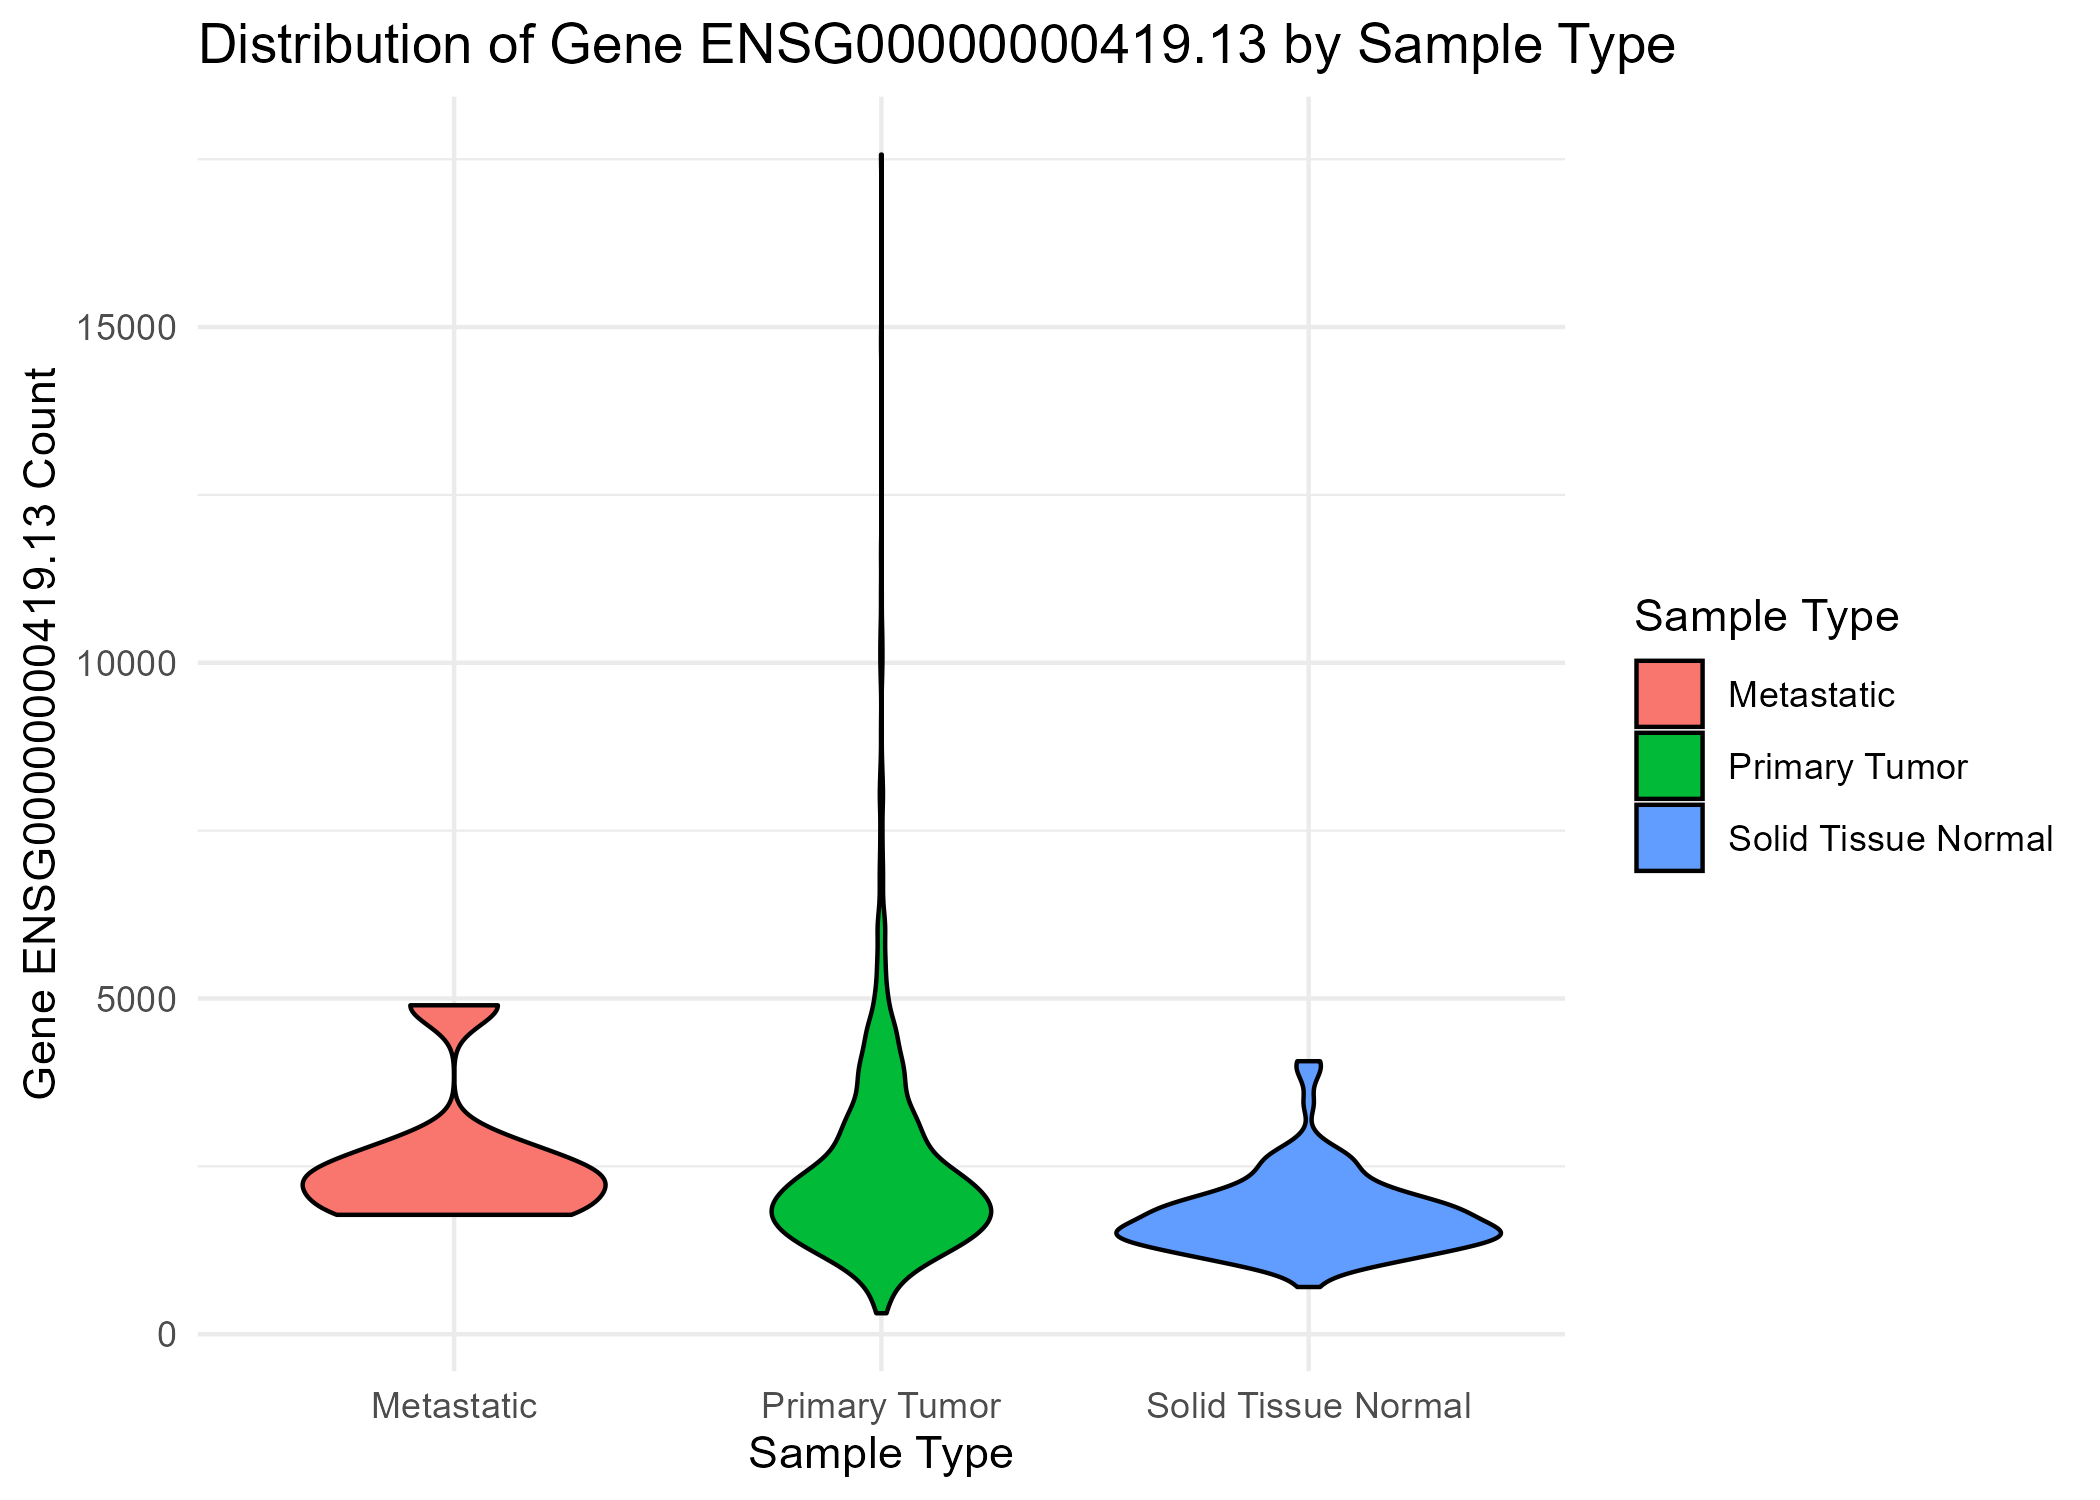
\includegraphics[width=0.5\textwidth]{final_project_violin.png}
    \caption{Distribution of Gene ENSG00000000419.13 by Sample Type.}
    \label{fig:violin}
\end{figure}

\subsection{Heatmap}
The heatmap visualized expression levels of \textbf{ten selected genes} across all samples, revealing distinct clusters corresponding to \textbf{sample type} categories. The top annotation bar provided clear differentiation among Metastatic, Primary Tumor, and Normal samples.
Each row represents a gene, and each column represents a sample. The color gradient (blue to red) indicates expression levels, where blue corresponds to low expression and red to high expression. Overall, the heatmap shows that Primary Tumor and Metastatic samples (orange and red bars) exhibit higher gene expression levels for several genes compared to Solid Tissue Normal samples (green bars), which remain mostly blue. Notably, genes like \textit{ENSG0000000419.13} show distinct upregulation in tumor samples, suggesting potential involvement in tumor development or progression.
\begin{figure}[H]
    \centering
    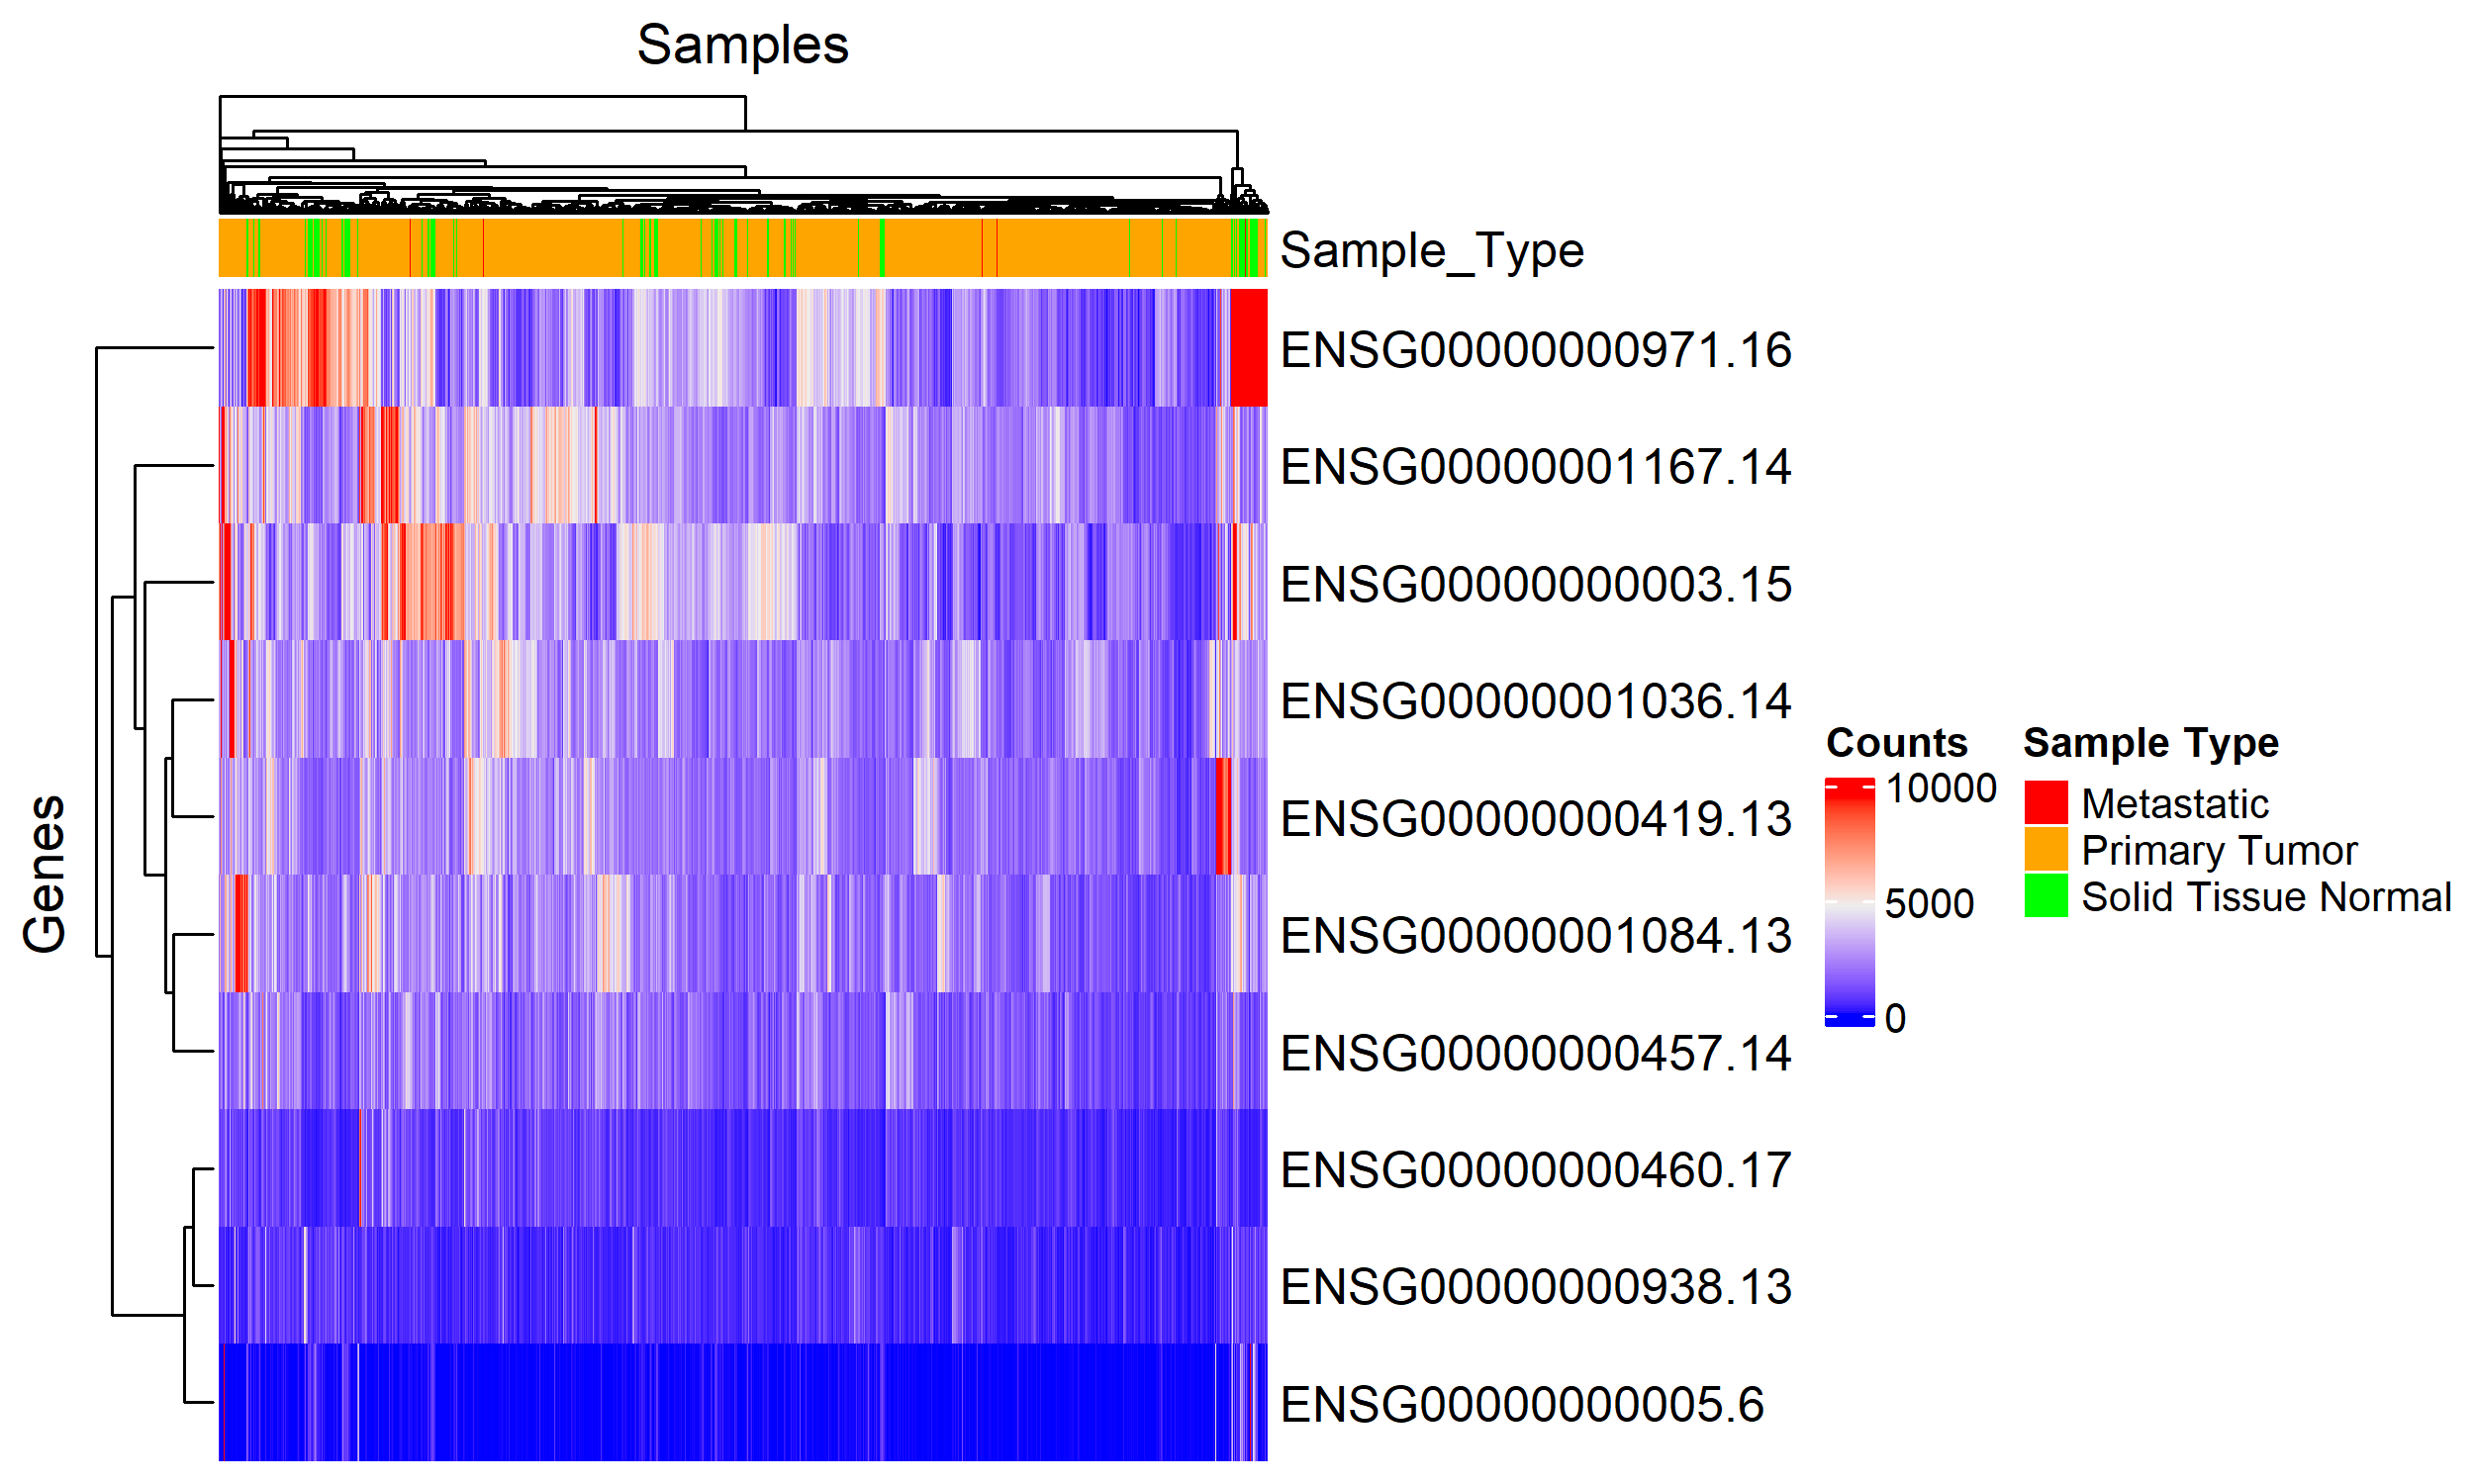
\includegraphics[width=0.6\textwidth]{final_project_heatmap.png}
    \caption{Heatmap of multiple gene expression profiles across sample types.}
    \label{fig:heatmap}
\end{figure}

\subsection{Bar Plot}
The bar chart displays the average expression of \textit{ENSG00000000419.13} by sample type. We see that \textbf{Metastatic} and \textbf{Primary Tumor} samples have \textbf{higher mean expression} compared to \textbf{Solid Tissue Normal}, indicating that this gene may be \textbf{upregulated in cancerous tissues} and could play a role in tumor development or progression. 

\begin{figure}[h]
    \centering
    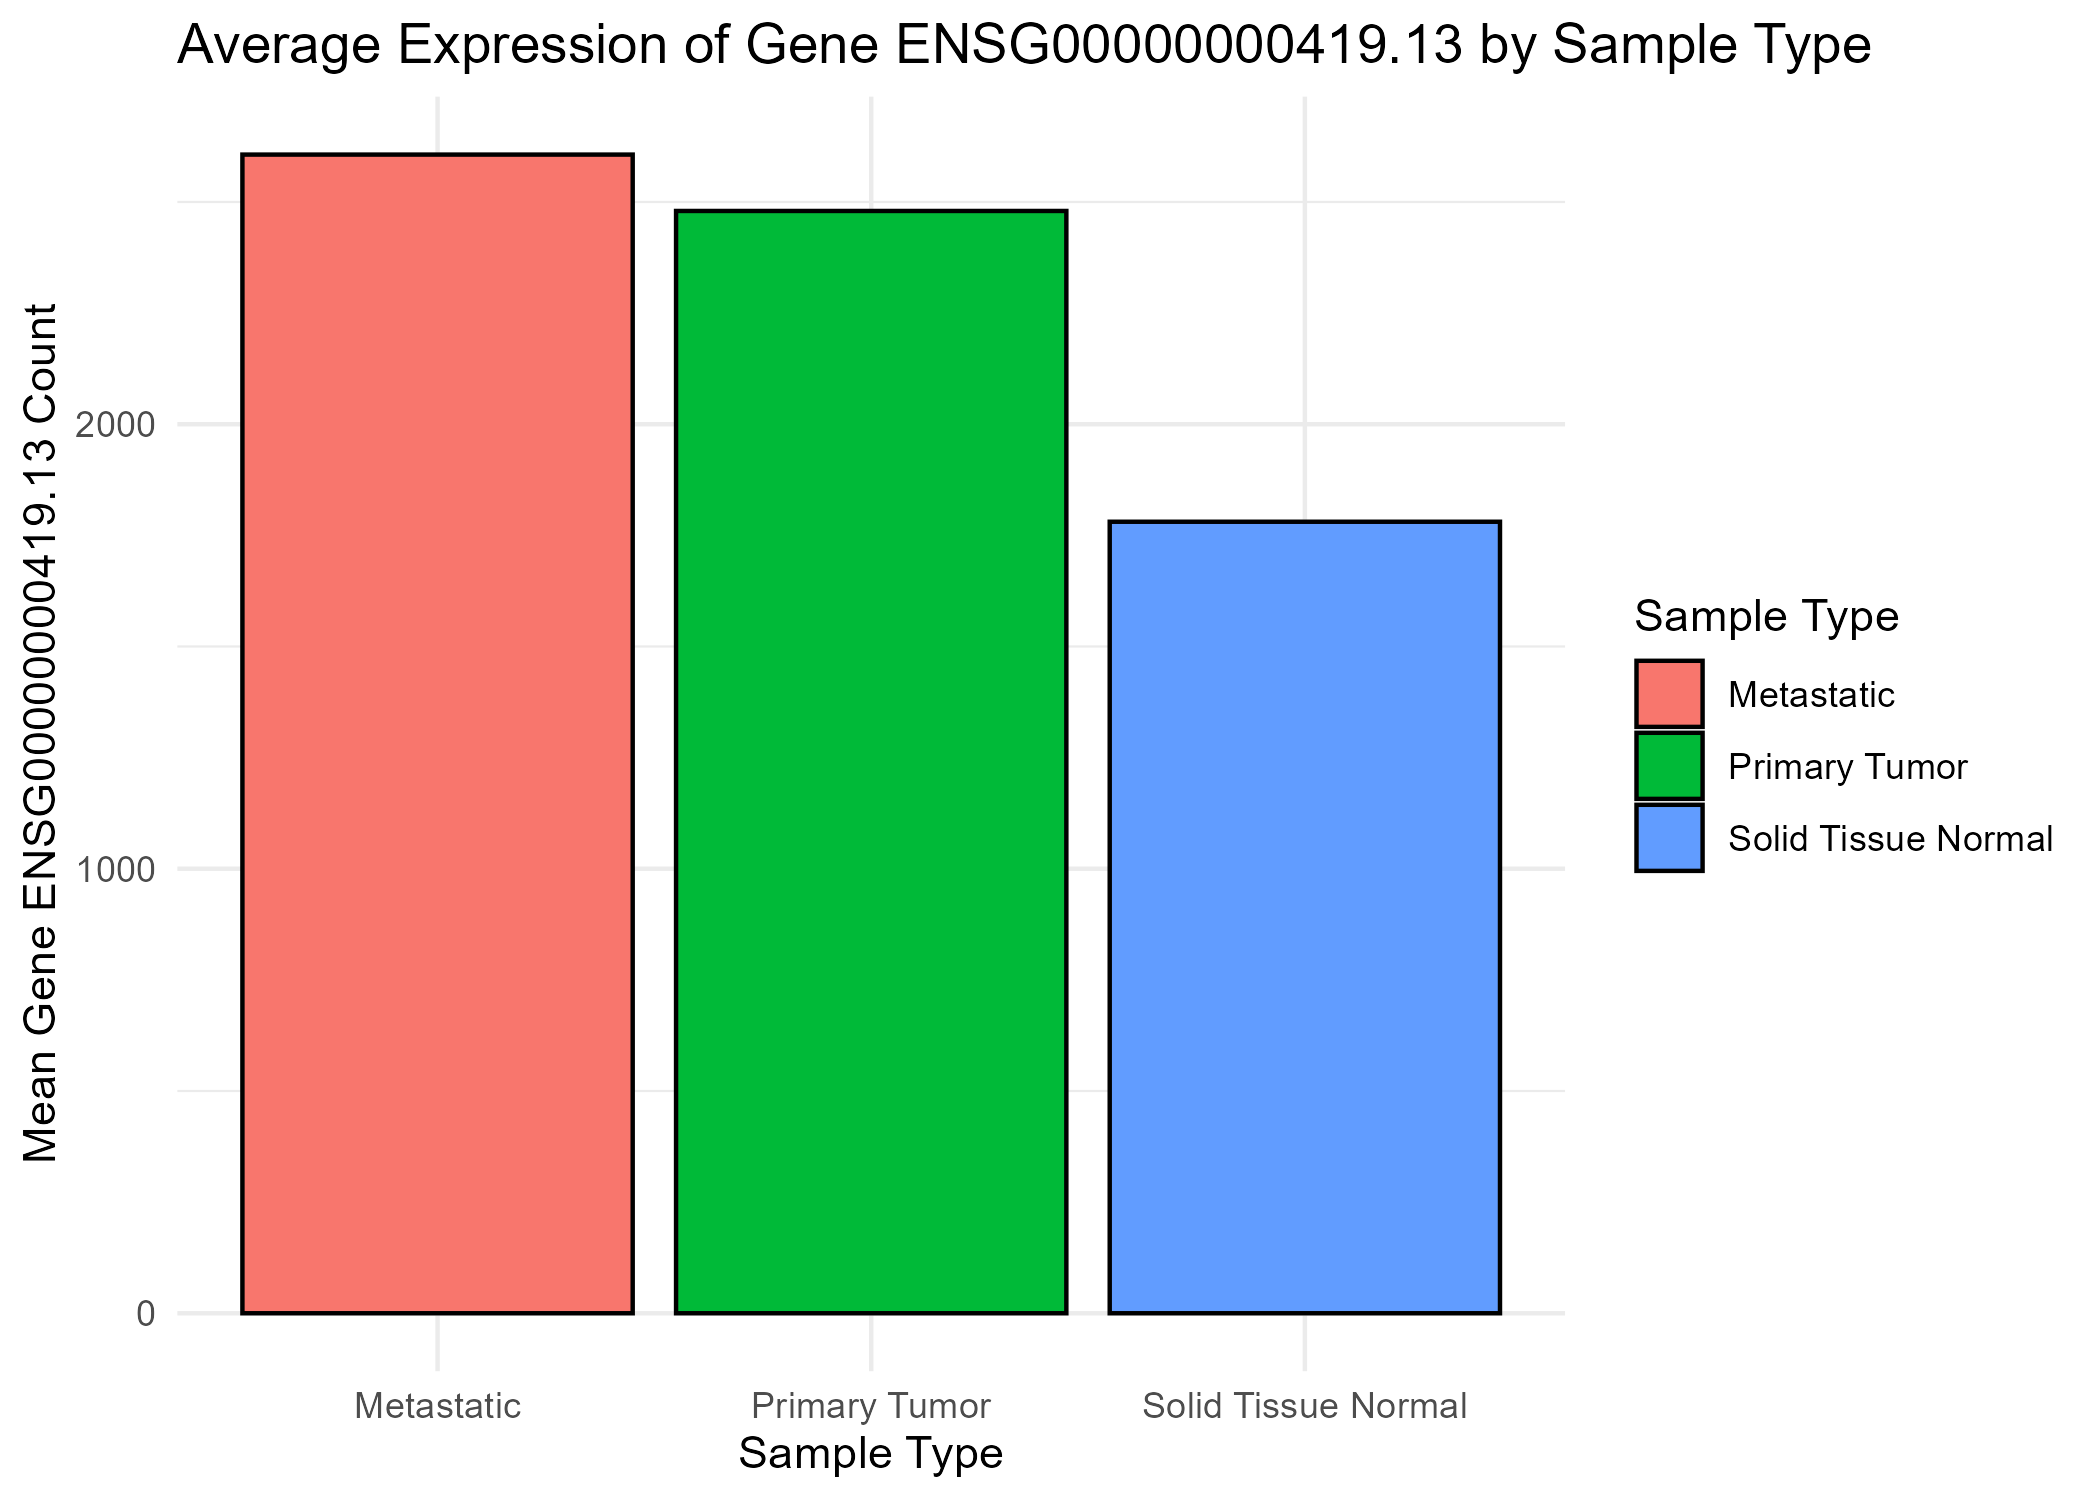
\includegraphics[width=0.5\textwidth]{final_project_bar_plot.png}
    \caption{Average expression of Gene ENSG00000000419.13 by sample type.}
    \label{fig:barplot}
\end{figure}

\subsection{Summary Statistics}
Summary statistics for both genes showed higher variability and mean values for \textit{ENSG00000000419.13} compared to \textit{ENSG00000000460.17}, consistent with its broader expression range across samples.



\begin{table}[ht]
\centering
\begin{tabular}{ |c|l|r|r| }
  \hline
 & Statistics & ENSG00000000419.13 & ENSG00000000460.17 \\ 
  \hline
1 & Mean & 2416.31 & 741.10 \\ \hline
  2 & Median & 2052.00 & 587.00 \\ \hline
  3 & Standard Deviation & 1459.49 & 627.80 \\ \hline
  4 & Minimum & 312.00 & 38.00 \\ \hline
  5 & Maximun & 17569.00 & 9377.00 \\ \hline
\end{tabular}
\caption{Summary Statistics of Gene ENSG00000000419.13 and ENSG00000000460.17} 
\end{table}



\section{References}
\begin{enumerate}
    \item Gu, Z. circlize implements and enhances circular visualization in R. Bioinformatics 2014.  
    \item R Core Team (2024). \textit{R: A language and environment for statistical computing}. R Foundation for Statistical Computing, Vienna, Austria. https://www.R-project.org/ 
    \item The Cancer Genome Atlas (TCGA). Retrieved from \url{https://portal.gdc.cancer.gov/}
    \item Wickham H (2016). \textit{ggplot2: Elegant Graphics for Data Analysis}. Springer-Verlag New York. ISBN 978-3-319-24277-4, https://ggplot2.tidyverse.org. 
\end{enumerate}
\end{document}
